%
% Nov. 10th:
% normalization, transformation and Gaussian theory parts has been carefully examined
%
%
%
%
%

\chapter{Basis Set Functions and Shell Pair Data}
%
%
%
In modern quantum chemistry package, usually there are two types of elementary functions
to compose the basis sets, one is the Slater type of function and the other is the 
Gaussian function. In our program, the basis set functions are all composed by Gaussian
type functions so that here the Gaussian functions is the only thing we are going to
talk.

The basis sets is usually composed by a set of Gaussian primitive functions. 
The Cartesian format has the form below:
\begin{equation}
 \label{int_sec1_eq:1}
  \chi = x^{l}y^{m}z^{n}e^{-\alpha r^{2}}
\end{equation}
and the spherical format has the form that:
\begin{equation}
 \label{int_sec1_eq:2}
\chi = r^{L}Y_{L}^{M}(\theta,\phi)e^{-\alpha r^{2}} 
\end{equation}
$Y_{L}^{M}$ is the spherical hamonic functions generated in the spherically symmetric 
potential(like for the atom system, so the spherical functions are more close to the
atom type of functions). we note that the angular momentum of L is expressed as 
$L = l + m + n$. Compared with the Cartesian format, the spherical
functions has less functions (2L+1) for a given angular momentum number (Cartesian functions 
has $(L+1)(L+2)/2$); hence the spherical functions are more useful in the calculation
involving higher angular momentum number.

For the basis set functions, it's usually expressed as linear combination of the 
Gaussian primitive functions on the same center; so that to mimic the atomic orbitals
for a given atom shell(S, P, D etc.):
\begin{equation}
 \label{int_sec1_eq:3}
  \phi_{i} = \sum_{j}d_{j}\chi_{ij}
\end{equation}
where the $d_{j}$ is some fixing constant.
In the following content, we use the $\chi$ to represent the Gaussian primitive 
functions, and to use $\phi$ to denote the basis set functions.

We are not going to give more talks related to the concepts and forming of the basis sets.
For this part of information, reader could refer to other materials for more information
\cite{Davidson_Feller_CR_86_681_1986} or see our previous chapter\ref{BASIS:2}.
Here in this chapter, we only describe the algorithms that how to handle the basis set
functions as well as shell pairs in the standard quantum chemistry software.  

The contents in this chapters are organized as below. Firstly, we will talke about the 
normalization for both primitives and the spherical primitives. Next, the transformation 
between the Cartesian type of functions into the spherical functions will be discussed 
in detail. Third, we will talk about the Gaussian product theorem, then based on this
theorem we will talk about what's the shell pair data and how to use it in the following
integral module.

%%%%%%%%%%%%%%%%%%%%%%%%%%%%%%%%%%%%%%%%%%%%%%%%%%%%%%%%%%%%%%%%%%%%%%%%%%%%%%%%%%%%%%%%%%%%%%%
\section{Normalization of Cartesian Basis Set Functions}
%
%
%
% 
The basis set functions of $\phi$, and the Gaussian primitive functions $\chi$ should be 
normalized before in use\footnote{This is necessary in the calculation. We can understand
it in this way, that in the final the wave function, each basis set/primitive should have
some proportion; such proportion is meaningful only if the component is normalized.}:
\begin{align}
 \label{int_sec2_eq:1}
\int \chi_{i}^{*}\chi_{i} dr &= 1 \nonumber \\
\int \phi_{\mu}^{*}\phi_{\mu} dr &= 1  
\end{align}

Firstly let's consider the normalization of the Gaussian primitive functions.  Suggest 
for a basis set function it's composed by uncontracted basis set functions,
which means we only have one primitive function in the basis function. Assuming we have a 
normalization constant of N for $\phi_{\mu}$, then we have:
\begin{align}
 \label{int_sec2_eq:2}
\int \phi_{\mu}^{*}\phi_{\mu} dr &= 
\int N^{2} (x^{l}y^{m}z^{n}e^{-\alpha r^{2}})(x^{l}y^{m}z^{n}e^{-\alpha r^{2}})
dxdydz \nonumber \\
&= N^{2} \int x^{2l}y^{2m}z^{2n}e^{-2\alpha r^{2}}dxdydz \nonumber \\
&=  N^{2} \int x^{2l}e^{-2\alpha x^{2}}dx\int y^{2m}e^{-2\alpha y^{2}}dy
\int z^{2n}e^{-2\alpha z^{2}}dz \nonumber \\
&=  N^{2} I_{x}I_{y}I_{z}
\end{align}
where I is\footnote{This is the integral for the Gamma function}:
\begin{equation}
 \label{int_sec2_eq:3}
I = \int^{-\infty}_{+\infty} x^{2k}e^{-2\alpha x^{2}}dx = 
\frac{(2k-1)!!\sqrt{\pi}}{(4\alpha)^{k}\sqrt{2\alpha}}
\end{equation}
Hence we can get that:
\begin{align}
 \label{int_sec2_eq:4}
N^{2}I_{x}I_{y}I_{z} &= 1 \nonumber \\
N &= \frac{1}{\sqrt{I_{x}I_{y}I_{z}}}  \nonumber \\
  &= \left( \frac{2}{\pi}\right)^{\frac{3}{4}} 
\frac{2^{l+m+n}\alpha^{\frac{2l+2m+2n+3}{4}}}{\sqrt{(2l-1)!!(2m-1)!!(2n-1)!!}}
\end{align}
This could be used in normalizing the Cartesian format of primitive functions.

Now let's step further to consider the contracted basis set functions:
\begin{equation}
  \label{int_sec2_eq:5}
\phi_{\mu} = \sum_{i}d_{\mu i}\chi_{i}
\end{equation}
For each basis set function, each component shares the same angular momentum part(
Physically each basis set function should be some simulation of the corresponding
atom orbitals). Hence we can expand the \ref{int_sec2_eq:5} into some detailed form:
\begin{align}
 \label{int_sec2_eq:6}
\phi_{\mu} &= \sum_{i}d_{\mu i}\chi_{i} \nonumber \\
&= \sum_{i}d_{\mu i} x^{l}y^{m}z^{n}e^{-\alpha r_{i}^{2}} 
\end{align}
Hence the \ref{int_sec2_eq:1} gives:
\begin{equation}
 \label{int_sec2_eq:7}
\begin{split}
 \int \phi_{\mu}^{*}\phi_{\mu} dr &= N^{2}\int x^{2l}y^{2m}z^{2n}
\left[ \sum_{i}d_{\mu i}e^{-\alpha r_{i}^{2}}\cdot\sum_{j}d_{\mu j}e^{-\alpha r_{j}^{2}}\right]
dr \\ 
&= N^{2}\sum_{i}\sum_{j}d_{\mu i}d_{\mu j}\int x^{2l}y^{2m}z^{2n}
e^{-\alpha (r_{i}+r_{j})^{2}} dr
\end{split}
\end{equation}
The result in the \ref{int_sec2_eq:7} can be easily calculated by extending \ref{int_sec2_eq:3}
into a new form (just to replace $2\alpha$ with $\alpha$):
\begin{equation}
 \label{int_sec2_eq:8}
\int x^{2k}e^{-\alpha x^{2}} dx = 
\frac{(2k-1)!!\sqrt{\pi}}{(2\alpha)^{k}\sqrt{\alpha}}
\end{equation}
Hence the integral for the \ref{int_sec2_eq:7} can be finally expressed as:
\begin{equation}
 \label{int_sec2_eq:9}
\int x^{2l}y^{2m}z^{2n}e^{-\alpha (r_{i}+r_{j})^{2}} = 
\frac{(2l-1)!!(2m-1)!!(2n-1)!!\pi^{\frac{3}{2}}}{2^{l+m+n}(\alpha_{i}+\alpha_{j})^{l+m+n+\frac{3}{2}}}
\end{equation}
Now we can get the final result:
\begin{align}
 \label{int_sec2_eq:10}
& N^{2}\frac{(2l-1)!!(2m-1)!!(2n-1)!!\pi^{\frac{3}{2}}}{2^{l+m+n}}
\sum_{i}\sum_{j}\frac{d_{\mu i}d_{\mu j}}{(\alpha_{i}+\alpha_{j})^{l+m+n+\frac{3}{2}}}
 = 1\rightarrow \nonumber \\
N &= \left[ 
\frac{(2l-1)!!(2m-1)!!(2n-1)!!\pi^{\frac{3}{2}}}{2^{l+m+n}}
\sum_{i}\sum_{j}\frac{d_{\mu i}d_{\mu j}}{(\alpha_{i}+\alpha_{j})^{l+m+n+\frac{3}{2}}} 
\right]^{-\frac{1}{2}}  
\end{align}

%%%%%%%%%%%%%%%%%%%%%%%%%%%%%%%%%%%%%%%%%%%%%%%%%%%%%%%%%%%%%%%%%%%%%%%%%%%%%%%%%%%%%%%%%%%%%%%
\section{Normalization for The Spherical Basis Set Functions}
%
%
%
Now let's concentrate on the normalization of an individual spherical primitive function
by start from the \ref{int_sec2_eq:1}:
\begin{equation}
 \begin{split}
  &N^{2}\int \chi_{i}^{*}\chi_{i} d\Omega = 1 \Longrightarrow  \\
  &N^{2}\int r^{L}Y_{L}^{M*}(\theta,\phi)e^{-\alpha r^{2}} 
r^{L}Y_{L}^{M}(\theta,\phi)e^{-\alpha r^{2}} d\Omega = 1  \\
&N^{2}\int_{0}^{\pi}\sin \theta d\theta \int_{0}^{2\pi}d\phi Y_{L}^{M*}(\theta,\phi)
Y_{L}^{M}(\theta,\phi) \int_{0}^{\infty} dr r^{2}r^{2L}e^{-2\alpha r^{2}} = 1
 \end{split}
\label{int_norm_eq:1}
\end{equation}
Since the $Y_{L}^{M}$ is the normalized form of function(will talk about in detail in
next section), hence they are orthogonal:
\begin{equation}
 \label{int_norm_eq:2}
\int_{0}^{\pi}\sin \theta d\theta \int_{0}^{2\pi}d\phi Y_{L^{'}}^{M^{'}*}(\theta,\phi)
Y_{L}^{M}(\theta,\phi) = \delta_{LL^{'}}\delta_{MM^{'}}
\end{equation}
Therefore the \ref{int_norm_eq:1} becomes:
\begin{equation}
 \begin{split}
  &N^{2}\int \chi_{i}^{*}\chi_{i} d\Omega = 1 \Longrightarrow  \\
  &N^{2}\int_{0}^{\infty} dr r^{2}r^{2L}e^{-2\alpha r^{2}} = 1
 \end{split}
\label{int_norm_eq:3}
\end{equation}

For the integral in \ref{int_norm_eq:3}, we have:
\begin{equation}
 \begin{split}
 \int_{0}^{\infty} dr r^{2}r^{2L}e^{-2\alpha r^{2}} &= 
\frac{2L+1}{4\alpha}\int_{0}^{\infty} dr r^{2L}e^{-2\alpha r^{2}}  \\
&=\frac{(2L+1)!!}{(4\alpha)^{L+1}}\int_{0}^{\infty} dr e^{-2\alpha r^{2}} \\
&=\frac{(2L+1)!!}{(4\alpha)^{L+1}}\frac{1}{2}\sqrt{\frac{\pi}{2\alpha}} \\
&=\frac{(2L+1)!!}{2^{2(L+1)+\frac{3}{2}}}\sqrt{\frac{\pi}{\alpha^{2L+3}}}
 \end{split}
\label{int_norm_eq:4}
\end{equation}
Therefore the normalization factor of $N$ is:
\begin{equation}
\label{int_norm_eq:5}
 N = \left[ \frac{(2L+1)!!}{2^{2(L+1)+\frac{3}{2}}}
            \sqrt{\frac{\pi}{\alpha^{2L+3}}}\right]^{-\frac{1}{2}}
\end{equation}
We can see that compared the \ref{int_norm_eq:5} with \ref{int_sec2_eq:4}, the normalization factor
for the spherical functions only depending on angular momentum. This is because we make use of 
the orthogonality condition of spherical harmonic of $Y_{L}^{M}$.

Now let's go to the contracted basis set functions:
\begin{equation}
 \label{int_norm_eq:6}
\phi_{\mu} = \sum_{i}d_{\mu i}\chi_{i}
\end{equation}
By repeating the same process, the result is:
\begin{equation}
 \begin{split}
&N^{2}\int \phi_{\mu}^{*}\phi_{\mu} dr =\\
& N^{2}\sum_{i}\sum_{j}d_{\mu i}d_{\mu j}
\int r^{L}Y_{L}^{M*}(\theta,\phi)e^{-\alpha_{i} r^{2}} 
r^{L}Y_{L}^{M}(\theta,\phi)e^{-\alpha_{j} r^{2}} d\Omega =   \\
&N^{2}\sum_{i}\sum_{j}d_{\mu i}d_{\mu j}
\int_{0}^{\infty} dr r^{2}r^{2L}e^{(\alpha_{i}+\alpha_{j}) r^{2}} \Rightarrow \\
&N =  \left[ \pi^{\frac{1}{2}}\frac{(2L+1)!!}{2^{(L+1)+1}}
\sum_{i}\sum_{j}\frac{d_{\mu i}d_{\mu j}}{(\alpha_{i}+\alpha_{j})^{L+\frac{3}{2}}}
\right]^{-\frac{1}{2}}
 \end{split}
\label{int_norm_eq:7}
\end{equation}


%%%%%%%%%%%%%%%%%%%%%%%%%%%%%%%%%%%%%%%%%%%%%%%%%%%%%%%%%%%%%%%%%%%%%%%%%%%%%%%%%%%%%%%%%%%%%%%
\section{Transformation from Cartesian Functions to Spherical functions}
\label{Transformation_Cart_sphere}
%
%
%
The core idea for the integral involving the spherical type of basis set functions, is that
we evaluate the integral first with its corresponding Cartesian type of functions. Then we 
transform it from Cartesian type into the spherical type. Since such transform is only related
to basis set itself, so the matrix is constant for any type of integrals (normalization, one 
electron integral and its derivatives etc.). In this section, we will discuss how to 
compute each element in the transformation matrix.

First of all, let's get to more familiar with the spherical harmonic function of 
$Y^{m}_{l}(\theta,\phi)$. This function is generated at any central field potential (which means,
the angular momentum operator is commuting with Hamiltonian for all of X, Y and Z direction). 
Typically,  any atom system is central field potential so that to describe the atomic orbital,
the spherical harmonic function is some necessary part. On the other hand, it's easy to see
that spherical harmonic function could be expanded into the sum over Cartesian type of functions;
therefore this is the reason that we could use the Cartesian type of function forming the basis 
set functions to mimic the atomic orbital.

The normalized $Y^{m}_{l}(\theta,\phi)$ used in this transformation could be expressed as
(here our derivation is normally just following Ref. \cite{QUA:QUA560540202}):
\begin{equation}
 \begin{split}
  Y^{m}_{l}(\theta,\phi) &= 
\sqrt{\frac{2l+1}{4\pi}\frac{(l-|m|)!}{(l+|m|)!}}e^{im\phi}P_{l}^{|m|}(\cos\theta) 
 \end{split}
\label{int_transform_pure_cart_eq:1}
\end{equation}
and we know that $m$ is between $-l$ and $+l$. $P_{l}^{|m|}(\cos\theta)$ is the 
associated Legendre polynomials, which expresses as (here we note this form is without
the Condon - Shortley phase factor of $(-1)^{m}$):
\begin{equation}
 \label{int_transform_pure_cart_eq:2}
\begin{split}
 P_{l}^{|m|}(\cos\theta) &= (1-\cos^{2}\theta)^{\frac{|m|}{2}}
\frac{\partial^{|m|}}{\partial\cos^{|m|}\theta}P_{l}(\cos\theta) \\
&= \frac{(1-\cos^{2}\theta)^{\frac{|m|}{2}}}{2^{l}l!}
\frac{\partial^{l+|m|}}{\partial\cos^{l+|m|}\theta}(\cos^{2}\theta-1)^{l}
\end{split}
\end{equation}

Here it's worthy to note, that why we use the $|m|$ rather than $m$ in the expression.
The associated Legendre polynomials satisfy the relation below($m > 0$):
\begin{equation}
 P_{l}^{-m}(\cos\theta) = (-1)^{m}\frac{(l-m)!}{(l+m)!}P_{l}^{m}(\cos\theta)
\end{equation}
therefore for the $Y^{m}_{l}(\theta,\phi)$ it satisfy:
\begin{equation}
 Y^{-m}_{l}(\theta,\phi) = (-1)^{m}Y^{m*}_{l}(\theta,\phi)
\end{equation}
and we also have:
\begin{equation}
 \int Y^{m*}_{l}(\theta,\phi) Y^{m^{'}}_{l^{'}}(\theta,\phi) d\theta d\phi = 
 \delta_{ll^{'}}\delta_{mm^{'}}
\end{equation}
Therefore, for simplicity here we could fix the $m$ to its absolute value:
\begin{equation}
\begin{split}
Y^{|m|}_{l}(\theta,\phi) &= 
\sqrt{\frac{2l+1}{4\pi}\frac{(l-|m|)!}{(l+|m|)!}}e^{im\phi} \\
&\frac{(1-\cos^{2}\theta)^{\frac{|m|}{2}}}{2^{l}l!}
\frac{\partial^{l+|m|}}{\partial\cos^{l+|m|}\theta}(\cos^{2}\theta-1)^{l} 
\end{split}
\label{int_transform_pure_cart_eq:3}
\end{equation}

Now let's try to convert the coordinates from spherical into the Cartesian. Firstly, 
we note that the above expression is for an arbitrary basis set function with 
spherical angular part. In practical use, we always stick to the normalized basis set
functions therefore we need to multiply the normalized factor\footnote{We note, that 
this is for normalized Cartesian type of functions. We assume that the basis set is
normalized, we need to drop the Cartesian normalization factor and multiply it with
the spherical normalization factor}:
\begin{equation}
 c = \frac{N_{spherical}}{N_{Cartesian}} c^{'}
\end{equation}
$c^{'}$ is the coefficients we will derive below, and $N_{spherical}$ is just the 
\ref{int_norm_eq:5}, and $N_{Cartesian}$ is just \ref{int_sec2_eq:4}. We note 
that $\dfrac{N_{spherical}}{N_{Cartesian}}$ is:
\begin{equation}
 \frac{N_{spherical}}{N_{Cartesian}} = \sqrt{\frac{4\pi 
 (2l_{x}-1)!!(2l_{y}-1)!!(2l_{z}-1)!!}{(2l+1)!!}}
\end{equation}
where we have $l = l_{x} + l_{y} + l_{z}$.

The \ref{int_transform_pure_cart_eq:3} is finally turned into:
\begin{equation}
\begin{split}
Y^{|m|}_{l}(\theta,\phi) &= 
\sqrt{\frac{(2l_{x})!(2l_{y})!(2l_{z})!l!}{(l_{x})!(l_{y})!(l_{z})!(2l)!}
\frac{(l-|m|)!}{(l+|m|)!}}e^{im\phi} \\
&\frac{(1-\cos^{2}\theta)^{\frac{|m|}{2}}}{2^{l}l!}
\frac{\partial^{l+|m|}}{\partial\cos^{l+|m|}\theta}(\cos^{2}\theta-1)^{l} 
\end{split}
\label{int_transform_pure_cart_eq:4}
\end{equation}

Now let's drop the partial derivatives in \ref{int_transform_pure_cart_eq:4} so that to 
expand it into the polynomials. In this process, since the factor of 
\begin{equation}
\sqrt{\frac{(2l_{x})!(2l_{y})!(2l_{z})!l!}{(l_{x})!(l_{y})!(l_{z})!(2l)!}
\frac{(l-|m|)!}{(l+|m|)!}}\frac{1}{2^{l}l!}
\end{equation}
is invariant therefore we designate it as $C$. Then the $Y^{m}_{l}(\theta,\phi)$ is:
\begin{equation}
 Y^{m}_{l}(\theta,\phi) = C
e^{im\phi}(1-\cos^{2}\theta)^{\frac{|m|}{2}}
\frac{\partial^{l+|m|}}{\partial\cos^{l+|m|}\theta}(\cos^{2}\theta-1)^{l}
\label{int_transform_pure_cart_eq:5}
\end{equation}

For the higher order partial derivatives, through binomial expression we can get:
\begin{equation}
\frac{\partial^{l+|m|}}{\partial\cos^{l+|m|}\theta}(\cos^{2}\theta-1)^{l} = 
\sum_{i=0}^{\left[ \frac{l-|m|}{2}\right]}\binom{l}{i}(-1)^{i}\frac{(2l-2i)!}{(l-|m|-2i)!}
\cos^{l-|m|-2i}\theta
\label{int_transform_pure_cart_eq:6}
\end{equation}

For the product between $e^{im\phi}(1-\cos^{2}\theta)^{\frac{|m|}{2}}$ we have:
\begin{equation}
 \begin{split}
 e^{im\phi}(1-\cos^{2}\theta)^{\frac{|m|}{2}} &=  
(\cos\phi\pm i\sin\phi)^{|m|}(\sin^{2}\theta)^{\frac{|m|}{2}} \\
&=\frac{1}{r^{|m|}\sin^{|m|}\theta}(x\pm iy)^{|m|}\sin^{|m|}\theta \\
&=\frac{(x \pm iy)^{|m|}}{r^{|m|}} 
 \end{split}
\label{int_transform_pure_cart_eq:7}
\end{equation}
Now multiply the $r^{l}$ the $Y^{m}_{l}$ becomes:
\begin{align}
 r^{l}Y^{m}_{l} &= C(x\pm iy)^{|m|}
\sum_{i=0}^{\left[ \frac{l-|m|}{2}\right] }
\binom{l}{i}(-1)^{i}\frac{(2l-2i)!}{(l-|m|-2i)!}\cos^{l-|m|-2i}\theta r^{l-|m|} \nonumber \\
&=  C(x\pm iy)^{|m|}
\sum_{i=0}^{\left[ \frac{l-|m|}{2}\right] }
\binom{l}{i}(-1)^{i}\frac{(2l-2i)!}{(l-|m|-2i)!}z^{l-|m|-2i}r^{2i}
\label{int_transform_pure_cart_eq:8}
\end{align}
Expanding the $r^{2i}$ gives:
\begin{equation}
\begin{split}
 r^{l}Y^{m}_{l} &=  C(x\pm iy)^{|m|}
\sum_{i=0}^{\frac{l-|m|}{2}}\binom{l}{i}(-1)^{i}\frac{(2l-2i)!}{(l-|m|-2i)!}z^{l-|m|-2i}r^{2i} \\
&= C(x\pm iy)^{|m|}
\sum_{i=0}^{\frac{l-|m|}{2}}\sum_{j=0}^{i} \\
&\binom{l}{i}\binom{i}{j}(-1)^{i}\frac{(2l-2i)!}{(l-|m|-2i)!}z^{l-|m|-2j}(x^{2}+y^{2})^{j}
\end{split}
\label{int_transform_pure_cart_eq:9} 
\end{equation}

Next we expand the $(x\pm iy)^{|m|}$ as well as $(x^{2}+y^{2})^{j}$:
\begin{equation}
 \begin{split}
 r^{l}Y^{m}_{l} &=  C(x\pm iy)^{|m|}
\sum_{i=0}^{\left[ \frac{l-|m|}{2}\right] }\sum_{j=0}^{i} \\
&\binom{l}{i}\binom{i}{j}(-1)^{i}\frac{(2l-2i)!}{(l-|m|-2i)!}z^{l-|m|-2j}(x^{2}+y^{2})^{j} \\
&= C\sum_{h=0}^{|m|}\sum_{i=0}^{\left[ \frac{l-|m|}{2}\right] }\sum_{j=0}^{i}\sum_{k=0}^{j} 
\binom{|m|}{h}\binom{l}{i}\binom{i}{j}\binom{j}{k} \\
&(-1)^{i}(\pm i)^{|m|-h}\frac{(2l-2i)!}{(l-|m|-2i)!} x^{2k+h}y^{|m|-h+2j-2k}z^{l-|m|-2j}
 \end{split}
\label{int_transform_pure_cart_eq:10} 
\end{equation}

Here we have the relation that:
\begin{equation}
 \begin{cases}
  2k+h &= l_{x}  \\
  |m|-h+2j-2k &= l_{y} \\
  l-|m|-2j &= l_{z}
 \end{cases}
\label{int_transform_pure_cart_eq:11} 
\end{equation}
Now the problem turns out to be that for a given set of $l_{x}, l_{y}$ and $l_{z}$; 
how we can determine the corresponding coefficient for the fixed l and m value.

Suggest that $l_{x}, l_{y}$ and $l_{z}$ are fixed, and $l = l_{x} + l_{y} + l_{z}$;
it could see that $j = (l-|m| - l_{z})/2$ and $h = l_{x} - 2k$. We note that the second 
function in \ref{int_transform_pure_cart_eq:11} is not independent. Therefore from 
\ref{int_transform_pure_cart_eq:10} we note the coefficient is:
\begin{equation}
 \begin{split}
  C_{r^{l}Y^{m}_{l}}^{l_{x}, l_{y}, l_{z}} &= C\sum_{i=0}^{\left[ \frac{l-|m|}{2}\right] }
\sum_{k=0}^{j} \\
&\binom{|m|}{l_{x}-2k}\binom{l}{i}\binom{i}{j}\binom{j}{k}(-1)^{i}(\pm i)^{|m|-l_{x}+2k}
\frac{(2l-2i)!}{(l-|m|-2i)!} \\
&= C\sum_{i=0}^{\left[ \frac{l-|m|}{2}\right] }
\sum_{k=0}^{j} \\
&\binom{|m|}{l_{x}-2k}\binom{l}{i}\binom{i}{j}\binom{j}{k}(-1)^{i}(-1)^{\frac{|m|-l_{x}+2k}{2}}
\frac{(2l-2i)!}{(l-|m|-2i)!} 
 \end{split}
\label{int_transform_pure_cart_eq:13} 
\end{equation}
Where 
\begin{equation}
 j = \left[ (l-|m| - l_{z})/2\right] 
\end{equation}
We could do more work so that to make the result in \ref{int_transform_pure_cart_eq:13}
more clear. If $j$ is not an integer, then the coefficient is zero. Furthermore 
in the original form  \ref{int_transform_pure_cart_eq:10} $j\leq i$ so if $j > i$ 
then the $\binom{i}{j} = 0$. For the $l_{x}-2k$, it meets the similar requirement that
$0\leq l_{x}-2k \leq |m|$ since the $l_{x}$ and $|m|$ are separate variables. In
the 
\ref{int_transform_pure_cart_eq:13}, if the $m<0$, we take ``-'' sing else we take ``+'' sign. 

In the real quantum chemistry package, actually we always stick to the real orbitals. However, 
we can always combine them into the real form:
\begin{align}
 C_{l,m,+}^{l_{x}, l_{y}, l_{z}} &= \frac{1}{\sqrt{2}}
\left( C_{r^{l}Y^{m}_{l}}^{l_{x}, l_{y}, l_{z}} + C_{r^{l}Y^{-m}_{l}}^{l_{x}, l_{y}, l_{z}}\right) 
\nonumber \\
 C_{l,m,-}^{l_{x}, l_{y}, l_{z}} &= \frac{-i}{\sqrt{2}}
\left( C_{r^{l}Y^{m}_{l}}^{l_{x}, l_{y}, l_{z}} - C_{r^{l}Y^{-m}_{l}}^{l_{x}, l_{y}, l_{z}}\right) 
\label{int_transform_pure_cart_eq:14}
\end{align}

%%%%%%%%%%%%%%%%%%%%%%%%%%%%%%%%%%%%%%%%%%%%%%%%%%%%%%%%%%%%%%%%%%%%%%%%%%%%%%%%%%%%%%%%%%%%%%%
\section{Transformation from Spherical functions to Cartesian functions}
\label{transformation_p2c}

Sometimes we will meet the reverse situation, that we need to convert the spherical functions
into the Cartesian ones. This is very common when we do integral calculation, since all of 
integrals are based on Cartesian form of Gaussian primitive functions.

Based on the expression for Cartesian to spherical transformation, this job is easily done.
Suppose we have an overlap matrix based on normalized Cartesian basis set functions, 
then we have the result below:
\begin{equation}
  \label{transformation_p2c_eq:1}
  T^{+}ST = I
\end{equation}
$T^{+}ST = I$ is because normalized spherical basis sets overlap matrix must give identity
matrix. $T$ is the transformation matrix to convert the overlap matrix from Cartesian 
into spherical type, and $T^{+}$ is it's conjugated matrix. Based on this idea,
the reverse of the $T$ could be simply expressed as:
\begin{equation}
 \label{transformation_p2c_eq:2}
 T^{+}ST = I \Rightarrow T^{-1} = T^{+}S 
\end{equation}
For $T$ with only real number, $T^{+}$ is simply the transpose of $T$.

Now the problem is that how can we calculate $S$. We can pick up the simplest form of basis
set functions. In these functions, there's only one only have one 
Gaussian primitive function, and all of the basis set functions are on same center. Furthermore,
all of these basis set functions have the same exponent factor
\footnote{Since the transformation work is independent on the 
basis set content, therefore we can choose to use the simplest basis set function to derive
the general formula here}. Based on our assumption, the basis set functions is simply expressed
as:
\begin{equation}
 \label{transformation_p2c_eq:3}
 \chi(r) = x^{l}y^{m}z^{n}e^{-\alpha r^{2}}
\end{equation}
For different basis set functions, only the $l,m,n$ change.

Now the matrix element in \ref{transformation_p2c_eq:1} can be expressed as:
\begin{equation}
 S_{ij} = N_{i}N_{j}\int\chi_{i}(r)\chi_{j}(r) dr = N_{i}N_{j}s_{ij}
\end{equation}
$N$ is the normalized factor for Cartesian basis set function.

Through the \ref{int_sec2_eq:4} we can get the normalized factor:
\begin{equation}
\label{transformation_p2c_eq:4}
N_{i} = \left( \frac{2}{\pi}\right)^{\frac{3}{4}} 
\frac{2^{l_{i}+m_{i}+n_{i}}\alpha^{\frac{2l_{i}+2m_{i}+2n_{i}+3}{4}}}
{\sqrt{(2l_{i}-1)!!(2m_{i}-1)!!(2n_{i}-1)!!}}
\end{equation}

The $s_{ij}$ can be got through \ref{overlap_direct_int_eq:9}:
\begin{align}
\int\chi_{i}(r)\chi_{j}(r) dr &= 
\int x^{l_{i}+l_{j}}y^{m_{i}+m_{j}}z^{n_{i}+n_{j}}e^{-(2\alpha)r^{2}} dr \nonumber \\
&= \left( \frac{\pi}{2\alpha}\right)^{\frac{3}{2}} 
\frac{(l_{i}+l_{j}-1)!!(m_{i}+m_{j}-1)!!(n_{i}+n_{j}-1)!!}
{(2(2\alpha))^{\frac{l_{i}+l_{j}+m_{i}+m_{j}+n_{i}+n_{j}}{2}}}
\end{align}

By setting that:
\begin{align}
 l_{i}+l_{j} &= l  \nonumber \\
 m_{i}+m_{j} &= m  \nonumber \\
 n_{i}+n_{j} &= n  \nonumber \\
 l_{i}+m_{i}+n_{i} &= l_{j}+m_{j}+n_{j} = L 
\end{align}
We can have:
\begin{align}
\label{transformation_p2c_eq:5}
 S_{ij} &= 
 \left( \frac{2}{\pi}\right)^{\frac{3}{4}} 
\frac{2^{L}\alpha^{\frac{2L+3}{4}}}{\sqrt{(2l_{i}-1)!!(2m_{i}-1)!!(2n_{i}-1)!!}} \times \nonumber \\
&\left( \frac{2}{\pi}\right)^{\frac{3}{4}} 
\frac{2^{L}\alpha^{\frac{2L+3}{4}}}{\sqrt{(2l_{j}-1)!!(2m_{j}-1)!!(2n_{j}-1)!!}} \times \nonumber \\
&\left( \frac{\pi}{2\alpha}\right)^{\frac{3}{2}} 
\frac{(l-1)!!(m-1)!!(n-1)!!}
{(4\alpha)^{L}} \nonumber \\
&= \frac{(l-1)!!(m-1)!!(n-1)!!}
{\sqrt{(2l_{i}-1)!!(2m_{i}-1)!!(2n_{i}-1)!!(2l_{j}-1)!!(2m_{j}-1)!!(2n_{j}-1)!!}}
\end{align}
This is what we need to know for the transformation process.

%%%%%%%%%%%%%%%%%%%%%%%%%%%%%%%%%%%%%%%%%%%%%%%%%%%%%%%%%%%%%%%%%%%%%%%%%%%%%%%%%%%%%%%%%%%%%%%
\section{Gaussian Primitive Product Theorem}
\label{Gaussian_Primitive_Product_Theorem}

Suggest that we have two arbitrary primitive functions, one is centered at nuclear A and the other
is centered at nuclear B; the electron is located at ``e'', which is shown by the figure \ref{fg:1}.
The theorem shows that for any two center Gaussian primitive functions, their product can be 
expressed by a new Gaussian type of primitive function which is centered at ``P''.

\begin{figure}[!hbp]
\begin{center}
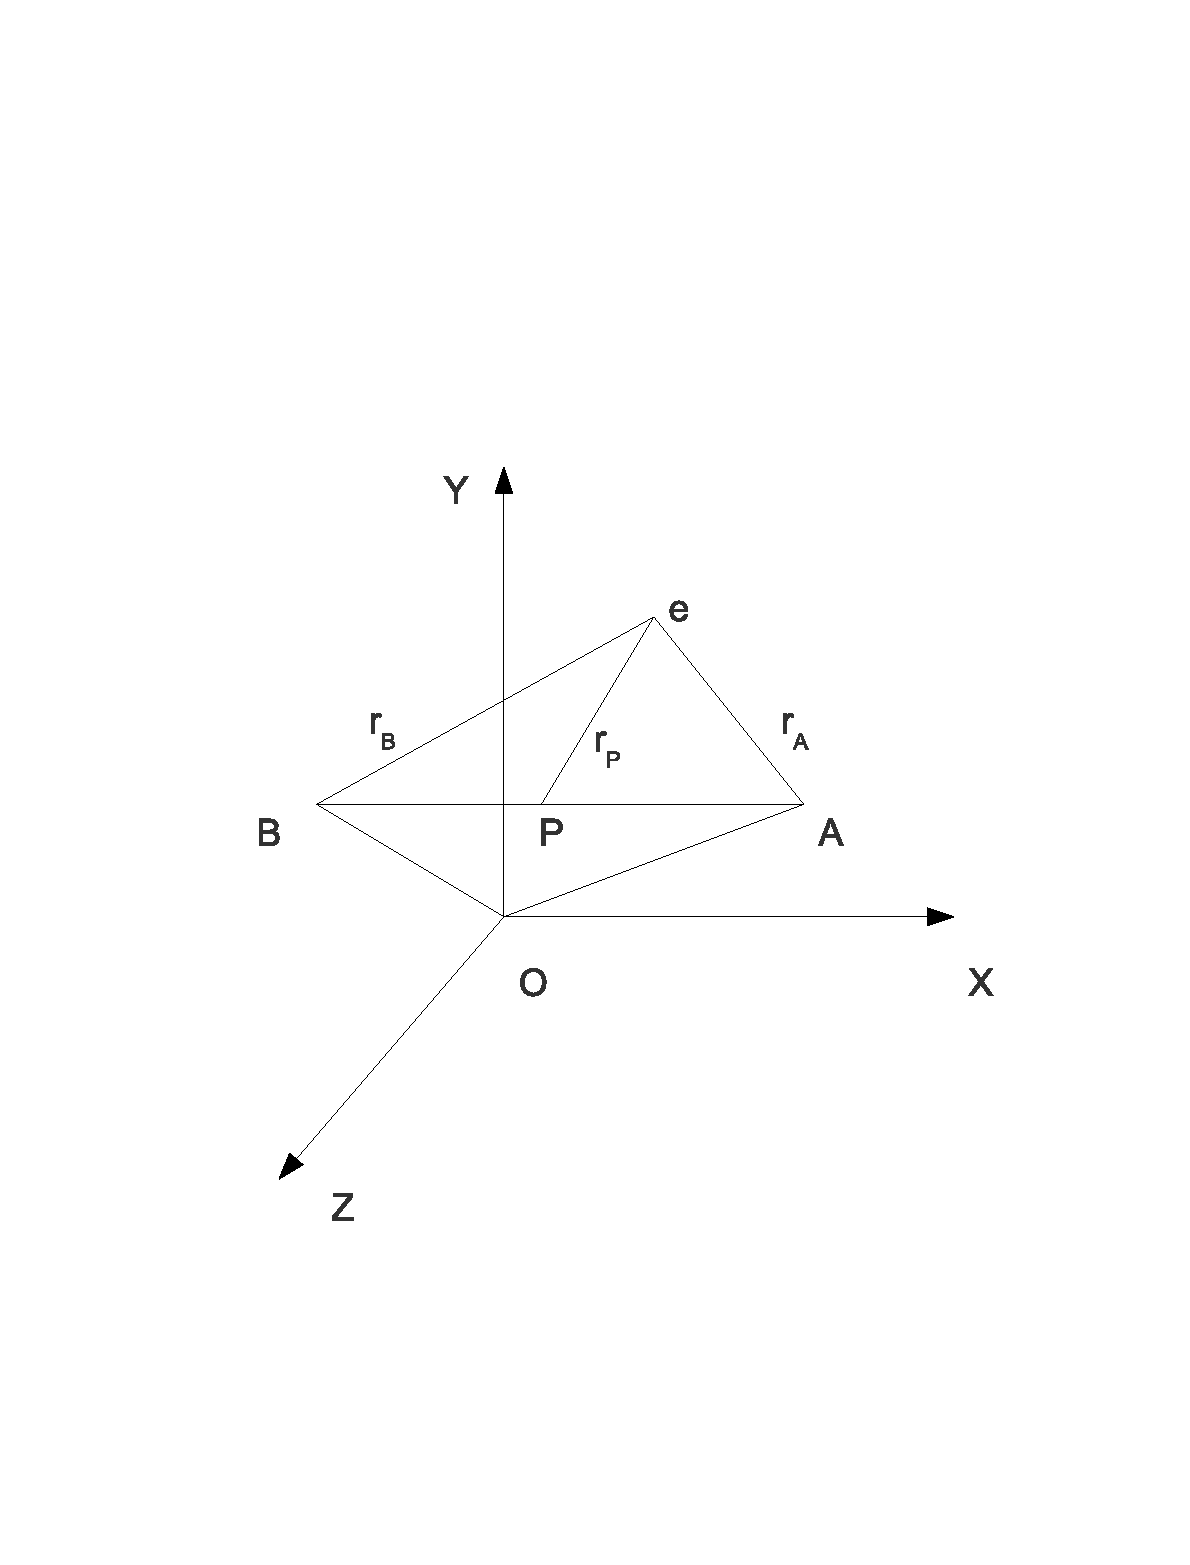
\includegraphics[scale=0.7]{gp.eps}
\caption{Gaussian primitive product theorem}
\label{fg:1}
\end{center}
\end{figure}

Now let's prove the simplest case, that both of the two primitive functions are S type of function; 
so the theorem can be stated as:
\begin{equation}
 \label{gaussian_product_rule_eq:1}
e^{-\alpha r_{A}^{2}}e^{-\beta r_{B}^{2}} = Ke^{-(\alpha+\beta) r_{P}^{2}}
\end{equation}
where $K$ is some constant.

Now let's prove it. By using the Cosine Rule, it's clear that:
\begin{align}
 \label{gaussian_product_rule_eq:2}
r_{A}^{2} &= r_{P}^{2} + \overline{PA}^{2} -2r_{P}\overline{PA}\cos\theta \nonumber \\
r_{B}^{2} &= r_{P}^{2} + \overline{PB}^{2} +2r_{P}\overline{PB}\cos\theta
\end{align}
Here $\theta$ is the angle formed by $\overline{AP}$ and $\overline{Pe}$.

Now let's get rid of the $\theta$. By multiplying $\overline{PB}$ to $r_{A}^{2}$, and 
multiplying $\overline{PA}$ to $r_{B}^{2}$ and add two equations in \ref{gaussian_product_rule_eq:2}
together; we can get:
\begin{equation}
 \label{gaussian_product_rule_eq:3}
\overline{PB}r_{A}^{2} + \overline{PA}r_{B}^{2} = \overline{AB}r_{P}^{2} + 
\overline{PA}\times\overline{PB}\times\overline{AB}
\end{equation}

However, in the exponent part of integral, besides the $r_{A}^{2}$ we have another factor 
of $\alpha$. Hence we have to find a way to associate the $\overline{PB}$ etc. with 
$\alpha$ so that to make up the exponent in the left hand side of \ref{gaussian_product_rule_eq:3}. 
It's easy to see that:
\begin{align}
 \label{gaussian_product_rule_eq:4}
\overline{PA} &= \frac{\beta}{\alpha+\beta}\overline{AB} \nonumber \\
\overline{PB} &= \frac{\alpha}{\alpha+\beta}\overline{AB}
\end{align}
Hence we can have:
\begin{equation}
\label{gaussian_product_rule_eq:5}
 \begin{split}
\frac{\alpha}{\alpha+\beta}\overline{AB}r_{A}^{2} +  
\frac{\beta}{\alpha+\beta}\overline{AB}r_{B}^{2} &= \overline{AB}r_{P}^{2} + 
\frac{\beta}{\alpha+\beta}\overline{AB}\frac{\alpha}{\alpha+\beta}\overline{AB}\times\overline{AB} 
 \end{split}
\end{equation}
Where we can get the result as:
\begin{equation}
\label{gaussian_product_rule_eq:6}
\alpha r_{A}^{2} + \beta r_{B}^{2} = (\alpha+\beta)r_{P}^{2} + \frac{\alpha\beta}{\alpha+\beta}
\overline{AB}^{2}
\end{equation}
Hence we have the final result as:
\begin{equation}
\label{gaussian_product_rule_eq:7}
e^{-\alpha r_{A}^{2} - \beta r_{B}^{2}} = 
e^{-(\alpha+\beta)r_{P}^{2}} e^{-\frac{\alpha\beta}{\alpha+\beta}
\overline{AB}^{2}}
\end{equation}

In the real calculation, it's necessary to know the P point location; that is to say, $P_{x}$ etc.
However, it's clear that the P's coordinate is determined by the $A$, $B$ and their exponents $\alpha$
and $\beta$:
\begin{equation}
 \label{gaussian_product_rule_eq:8}
\begin{split}
 \overline{PA} &= \frac{\beta}{\alpha+\beta}\overline{BA} \rightarrow \\
\overrightarrow{P} - \overrightarrow{A} &= \frac{\beta}{\alpha+\beta}
(\overrightarrow{B} - \overrightarrow{A}) \rightarrow  \\
\overrightarrow{P} &= \frac{\alpha}{\alpha+\beta}\overrightarrow{A} + 
\frac{\beta}{\alpha+\beta}\overrightarrow{B}
\end{split}
\end{equation}
So from here all of $P_{x}$, $P_{y}$ and $P_{z}$ can be got.

Now let's extend it to any arbitrary Gaussian primitives, that is to say; how we can express 
the following expression?
\begin{equation}
   x_{A}^{l_{1}}y_{A}^{m_{1}}z_{A}^{n_{1}}e^{-\alpha r_{A}^{2}}
   x_{B}^{l_{2}}y_{B}^{m_{2}}z_{B}^{n_{2}}e^{-\beta  r_{B}^{2}}   =  ?
\label{gaussian_product_rule_eq:9}
\end{equation}
for the $X_{A}$, since we have:
\begin{equation}
\begin{split}
 x_{A} &= e_{x} - A_{x} \\
       &= e_{x} - P_{x} + P_{x} - A_{x} \\
       &= x_{P} + \overline{PA}_{x} 
\end{split}
 \label{gaussian_product_rule_eq:10}
\end{equation}
Hence for the $x_{A}$ it totally converts into the expression related to $x_{P}$.

Similarly, for the $y_{A}$, $z_{A}$ etc. it's convenient to get their expressions too. So we can
finally convert the \ref{gaussian_product_rule_eq:9} into:
\begin{align}
&  x_{A}^{l_{1}}y_{A}^{m_{1}}z_{A}^{n_{1}}e^{-\alpha r_{A}^{2}}
   x_{B}^{l_{2}}y_{B}^{m_{2}}z_{B}^{n_{2}}e^{-\beta  r_{B}^{2}} \nonumber \\
=& (x_{P} + \overline{PA}_{x})^{l_{1}}(y_{P} + \overline{PA}_{y})^{m_{1}}
   (z_{P} + \overline{PA}_{z})^{n_{1}}e^{-\alpha r_{A}^{2}} \times \nonumber \\
&  (x_{P} + \overline{PB}_{x})^{l_{2}}(y_{P} + \overline{PB}_{y})^{m_{2}}
   (z_{P} + \overline{PB}_{z})^{n_{2}}e^{-\beta  r_{B}^{2}} \nonumber \\
=& (x_{P} + \overline{PA}_{x})^{l_{1}}(y_{P} + \overline{PA}_{y})^{m_{1}}
   (z_{P} + \overline{PA}_{z})^{n_{1}} \times \nonumber \\
&  (x_{P} + \overline{PB}_{x})^{l_{2}}(y_{P} + \overline{PB}_{y})^{m_{2}}
   (z_{P} + \overline{PB}_{z})^{n_{2}} \times \nonumber \\
&  e^{-(\alpha+\beta)r_{P}^{2}} e^{-\frac{\alpha\beta}{\alpha+\beta}
\overline{AB}^{2}}
  \label{gaussian_product_rule_eq:11}
\end{align}

In the practical calculation, usually it's required to separate the $x_{P}$ etc. from the 
$(x_{P} +\overline{PA}_{x})^{l_{1}}$. So according to binomial theorem we may have:
\begin{equation}
 (x_{P} +\overline{PA}_{x})^{l_{1}} = \sum_{i=0}^{l_{1}} x_{P}^{i}\overline{PA}_{x}^{l_{1}-i}
\binom{l_{1}}{i}
 \label{gaussian_product_rule_eq:12}
\end{equation}

Hence we could combine the two terms together:
\begin{equation}
\label{gaussian_product_rule_eq:13}
\begin{split}
(x_{P} +\overline{PA}_{x})^{l_{1}}(x_{P} + \overline{PB}_{x})^{l_{2}}
&=  \sum_{i=0}^{l_{1}} x_{P}^{i}\overline{PA}_{x}^{l_{1}-i}
\binom{l_{1}}{i}
    \sum_{j=0}^{l_{2}} x_{P}^{j}\overline{PB}_{x}^{l_{2}-j}
\binom{l_{2}}{j} \\
&= \sum_{k=0}^{l_{1}+l_{2}}x_{P}^{k}
\sum_{i=0,j=k-i}^{i=l_{1},j=l_{2}}\overline{PA}_{x}^{l_{1}-i}
\overline{PB}_{x}^{l_{2}-j}\binom{l_{1}}{i}\binom{l_{2}}{j}
\end{split}
\end{equation}

Now let's make some further analysis to the result shown in the \ref{gaussian_product_rule_eq:13}.
The term involves $i,j$ together actually is not convenient for computation purpose, hence we should
make it easier. Firstly we noticed that for the index $i$ we have such restrictions:
\begin{equation}
 \begin{cases}
  &0 \leq i \leq l_{1} \\
  &k-l_{2} \leq i \leq k
 \end{cases}
\end{equation}
$i\leq k$ is because that $i+j=k$ and $j\geq 0$. $i\geq k-l_{2}$ is because $l_{2} - k+i \geq 0$ in 
the \ref{gaussian_product_rule_eq:13}. Therefore the problem here is how can we sort out the 
real range of $i$?

Now we can guess that \ref{gaussian_product_rule_eq:13} perhaps can be rearranged into the form 
below\footnote{In practice we have tested the expression below for the $(x+a)^{3}(x+b)^{2}$, but
the proof can demonstrate that it's true for all of cases}:
\begin{multline}
\label{gaussian_product_rule_eq:14}
 (x_{P} +\overline{PA}_{x})^{l_{1}}(x_{P} + \overline{PB}_{x})^{l_{2}} = \\
\sum_{k=0}^{l_{1}+l_{2}}x_{P}^{k} 
\sum_{i=max(0,k-l_{2})}^{i=min(k,l_{1})}\overline{PA}_{x}^{l_{1}-i}
\overline{PB}_{x}^{l_{2}-k+i}\binom{l_{1}}{i}\binom{l_{2}}{k-i}
\end{multline}

Now let's literally prove it. Suggest we have the expression below:
\begin{align}
\label{gaussian_product_rule_eq:15}
 (x_{P} +\overline{PA}_{x})^{l_{1}}(x_{P} + \overline{PB}_{x})^{l_{2}} &= 
\sum_{i=0}^{l_{1}} x_{P}^{i}\overline{PA}_{x}^{l_{1}-i}
\binom{l_{1}}{i}
    \sum_{j=0}^{l_{2}} x_{P}^{j}\overline{PB}_{x}^{l_{2}-j}
\binom{l_{2}}{j} \nonumber \\
&=\sum_{k=0}^{l_{1}+l_{2}}x_{P}^{k} f_{k}(i,j,l_{1},l_{2},\overline{PA}_{x},\overline{PB}_{x})
\end{align} 
Where $i+j = k$, and $f_{k}$ expressed as:
\begin{equation}
\label{gaussian_product_rule_eq:16}
 f_{k}(i,j,l_{1},l_{2},\overline{PA}_{x},\overline{PB}_{x}) = 
\sum_{?}^{?}
\overline{PA}_{x}^{l_{1}-i}
\overline{PB}_{x}^{l_{2}-j}\binom{l_{1}}{i}\binom{l_{2}}{j}
\end{equation}

It's easy to know, that for each fixed $k$ value, $(i=0,j=k), (i=1,j=k-1), \cdots, 
(i=k,j=0)$ contribute to the $f_{k}$. However, since $i$ and $j$ are also limited by the 
$l_{1}$ and $l_{2}$, the $i$ and $j$ may not be able to take all of the pairs shown before.  
Now the problem is, if we very $i$ freely, and take $j=k-i$; then what's the range of $i$
in variation? 

Firstly let's consider the starting point of $i$. Obviously $i$ could start from $0$, however;
if $i=0$, then for a fixed $k$ then $j$ is $j=k-0=k$. But $j$ has a upper limit which is 
$j\leq l_{2}$, and it could have the situation that $l_{2} \leq k$. Hence in this situation, 
where $l_{2} \leq k$, then the minimum value of $i$ could not be $0$, but the value of $k-l_{2}$
since the maximum value of $j$ is $l_{2}$. The analysis here indicates that for the starting 
point of $i$, we should use ``max'' function for the $(0, k-l_{2})$.

Second let's go to see the end point of $i$. The $i$ could be $l_{1}$ from its definition,
however; as $i=l_{1}$ then $j=k-i=k-l_{1}$ that we may have the situation of $k-l_{1}\leq 0$.
Since $j$ must be larger or equal to zero so that the maximum number of $i$ could be $k$ 
(if $l_{1}\geq k$) or could be $l_{i}$ (if $l_{1}\leq k$). In this case, we have a minimum 
function of ``min'' between $(k,l_{1})$.

Finally, we note that the range analysis does not change the mathematical expression in the 
\ref{gaussian_product_rule_eq:16}. Hence the proof is ended. 

Now in the \ref{gaussian_product_rule_eq:16}, we are going to drop the index of $i$, $j$ from
the $f_{k}$ variable list since $i$ is summed over in the expression, and $j=k-i$ so that solely
determined by $i$ and $k$; hence we have:
\begin{equation}
\label{gaussian_product_rule_eq:17}
 (x_{P} +\overline{PA}_{x})^{l_{1}}(x_{P} + \overline{PB}_{x})^{l_{2}} = 
\sum_{k=0}^{l_{1}+l_{2}}x_{P}^{k}f_{k}(l_{1},l_{2},\overline{PA}_{x},\overline{PB}_{x}) 
\end{equation}
and $f_{k}$ is:
\begin{equation}
 \label{gaussian_product_rule_eq:18_0}
f_{k}(l_{1},l_{2},\overline{PA}_{x},\overline{PB}_{x}) = 
\sum_{i=max(0,k-l_{2})}^{i=min(k,l_{1})}\overline{PA}_{x}^{l_{1}-i}
\overline{PB}_{x}^{l_{2}-k+i}\binom{l_{1}}{i}\binom{l_{2}}{k-i}
\end{equation}

The expression in the \ref{gaussian_product_rule_eq:18} actually only applies for the situation 
that both $l_{1}$ and $l_{2}$ larger than zero. For the cases that $l_{1}$ or $l_{2}$ equal to zero,
we can directly use the binomial theorem to get the result. Hence the final result for the 
$f_{k}$ could be expressed as:
\begin{align}
\label{gaussian_product_rule_eq:18}
 &f_{k}(l_{1},l_{2},\overline{PA}_{x},\overline{PB}_{x}) \nonumber \\
&=
\begin{cases}
\sum_{i=max(0,k-l_{2})}^{i=min(k,l_{1})}\overline{PA}_{x}^{l_{1}-i}
\overline{PB}_{x}^{l_{2}-k+i}\binom{l_{1}}{i}\binom{l_{2}}{k-i}
    & l_{1} > 0, l_{2} > 0 \\
\overline{PA}_{x}^{l_{1}-k}\binom{l_{1}}{k}  
&  l_{1} > 0, l_{2} = 0 \\
\overline{PB}_{x}^{l_{2}-k}\binom{l_{2}}{k}  
&  l_{1} = 0, l_{2} > 0 \\
1                                           
&  l_{1} = 0, l_{2} = 0
\end{cases}
\end{align} 

Based on this result, for two arbitrary Gaussian primitives product on different center; 
we have the result as:
\begin{align}
&  x_{A}^{l_{1}}y_{A}^{m_{1}}z_{A}^{n_{1}}e^{-\alpha r_{A}^{2}}
   x_{B}^{l_{2}}y_{B}^{m_{2}}z_{B}^{n_{2}}e^{-\beta  r_{B}^{2}} \nonumber \\
=& \sum_{i=0}^{l_{1}+l_{2}}x_{P}^{i}f_{i}(l_{1},l_{2},\overline{PA}_{x},\overline{PB}_{x})  
   \times \nonumber \\
 & \sum_{j=0}^{m_{1}+m_{2}}y_{P}^{j}f_{j}(m_{1},m_{2},\overline{PA}_{y},\overline{PB}_{y})  
   \times \nonumber \\
 & \sum_{k=0}^{n_{1}+n_{2}}z_{P}^{k}f_{k}(n_{1},n_{2},\overline{PA}_{z},\overline{PB}_{z})  
   \times \nonumber \\
 &  e^{-(\alpha+\beta)r_{P}^{2}} e^{-\frac{\alpha\beta}{\alpha+\beta}\overline{AB}^{2}}
   \Rightarrow \nonumber \\
 & =\sum_{i=0}^{l_{1}+l_{2}}\sum_{j=0}^{m_{1}+m_{2}}\sum_{k=0}^{n_{1}+n_{2}}
   x_{P}^{i}y_{P}^{j}z_{P}^{k}
   e^{-(\alpha+\beta)r_{P}^{2}} e^{-\frac{\alpha\beta}{\alpha+\beta}\overline{AB}^{2}}
   \times F_{ijk}
  \label{gaussian_product_rule_eq:19}
\end{align}
Where $F_{ijk}$ is:
\begin{multline}
  F_{ijk} = \\
            f_{i}(l_{1},l_{2},\overline{PA}_{x},\overline{PB}_{x})
            f_{j}(m_{1},m_{2},\overline{PA}_{y},\overline{PB}_{y})
            f_{k}(n_{1},n_{2},\overline{PA}_{z},\overline{PB}_{z}) 
 \label{gaussian_product_rule_eq:20}
\end{multline}

Finally we note that for the same center situation, things is much more easier:
\begin{align}
&  x_{A}^{l_{1}}y_{A}^{m_{1}}z_{A}^{n_{1}}e^{-\alpha r_{A}^{2}}
   x_{A}^{l_{2}}y_{A}^{m_{2}}z_{A}^{n_{2}}e^{-\beta  r_{A}^{2}} \nonumber \\
=& x_{A}^{l_{1}+l_{2}}y_{A}^{m_{1}+m_{2}}z_{A}^{n_{1}+n_{2}}e^{-(\alpha+\beta)r_{A}^{2}}
  \label{gaussian_product_rule_eq:21}
\end{align} 


%%%%%%%%%%%%%%%%%%%%%%%%%%%%%%%%%%%%%%%%%%%%%%%%%%%%%%%%%%%%%%%%%%%%%%%%%%%%%%%%%%%%%%%%%%%%%%%%
\section{Shell Pair Data}
%
%
%
%
The Gaussian Primitive Product Theorem plays an key role in quantum chemistry\cite{SFBoys1950}. This
theorem is the key to understand that why we introduce the Gaussian type functions into the quantum 
chemistry; after all, the Slater type of function is more like the real wave function for atom system.
However, the integral for STO is too expensive to evaluate so that  we can use the linear combination 
of Gaussian functions to imitate the Slater functions, then to simulate the wave functions for atom.
Such idea is the crucial point for building the basis sets which is generally used in quantum chemistry
package.

In quantum chemistry, the electron integral could be generally expressed as:
\begin{equation}
 \label{shell_pair_eq:1}
I = \sum_{i=1}^{K}\sum_{j=1}^{K}\sum_{k=1}^{K}\sum_{l=1}^{K}
\int \int \chi_{i}^{*}(r)\chi_{j}^{*}(r)f(r,r^{'})
\chi_{k}(r^{'})\chi_{l}(r^{'}) dr dr^{'}
\end{equation}
Here $\chi$ is the Gaussian primitive function with arbitrary angular momentum, and $f(r,r^{'})$ is the 
electron operator for one or two electrons. Generally through the Gaussian Primitive Product Theorem, 
we could firstly combine the $ \chi_{i}^{*}(r)\chi_{j}^{*}(r)$ together into a new Gaussian function, 
so as for the $\chi_{k}(r^{'})\chi_{l}(r^{'})$. Therefore, the integral has been simplified into some
new form which only has two Gaussian functions.

Formally, we could designate the $ \chi_{i}^{*}(r)\chi_{j}^{*}(r)$ as ``shell pair'', which is 
physically related to the electron density (when multiply with MO coefficients etc.):
\begin{align}
\label{shell_pair_eq:2}
 \chi_{i}^{*}(r)\chi_{j}^{*}(r) \Longrightarrow (ij| \nonumber \\
 \chi_{k}(r^{'})\chi_{l}(r^{'}) \Longrightarrow |kl)
\end{align}
Such concept is trivial physically, but could bring great benefit for designing the software. 
Therefore, any analytical electron integrals we discuss later will be realized based on the shell pair
data.
    

%%%%%%%%%%%%%%%%%%%%%%%%%%%%%%%%%%%%%%%%%%%%%%%%%%%%%%%%%%%%%%%%%%%%%%%%%%%%%%%%%%%%%%%%%%%%%%%%
\section{Hermite Polynomials in Shell Pair Data}
%
%
%
%
In section \label{Gaussian_Primitive_Product_Theorem}, we have derived the shell pair data as:
\begin{equation}
\label{basic_shell_pair_data_form}
 |\chi_{A}\chi_{B}) = 
\begin{cases}
 \sum_{i=0}^{l_{1}+l_{2}}\sum_{j=0}^{m_{1}+m_{2}}\sum_{k=0}^{n_{1}+n_{2}}
   x_{P}^{i}y_{P}^{j}z_{P}^{k}
   e^{-(\alpha+\beta)r_{P}^{2}} e^{-\frac{\alpha\beta}{\alpha+\beta}\overline{AB}^{2}}
   \times F_{ijk}  \\
 x_{A}^{l_{1}+l_{2}}y_{A}^{m_{1}+m_{2}}z_{A}^{n_{1}+n_{2}}e^{-(\alpha+\beta)r_{A}^{2}}
\end{cases}
\end{equation}
It turns out that the complexity behind the shell pair data is brought by the angular momentum part.
For some arbitrary angular momentum number, each combination will introduce three sums hence
for two electron integral at least six round of sums is needed. Therefore, it implies that the 
angular momentum is the potential bottle neck for the integral evaluation.

Is there any way to avoid direct calculation of angular momentum part? Physically, the angular 
momentum part for atom wave function is generated by the central field; which turns out to be 
in form of $Y^{m}_{l}(\theta,\phi)$, and this is a set of orthogonal functions(see 
\ref{Transformation_Cart_sphere} for more information). Therefore, it implies that we could also
express the angular momentum part into other set of orthogonal functions (here we may need some
transformation, which finally convert it back to the Cartesian form or spherical form of 
basis set functions). The new form of basis set functions may bring us extra benefit in calculating
the integrals.
 
McMurchie and Davidson showed that\cite{MD} it's possible to use the
Hermite polynomials to achieve such transformation. Typically, they defined the
new angular momentum part in the Gaussian primitive functions as:
\begin{equation}
 \label{Shell_pair_data_further_eq:1}
\Lambda_{n}(\alpha, x_{p}) = e^{\alpha x_{p}^{2}} \frac{\partial^{n}}{\partial
P_{X}^{n}}\left( e^{-\alpha x_{p}^{2}} \right) 
\end{equation}
Here $x_{p}$ is defined the same as in \ref{gaussian_product_rule_eq:10}, which
is $x_{p} = e_{x} - P_{x}$. Now with the transformation that
\begin{equation}
 \label{Shell_pair_data_further_eq:2}
\frac{\partial}{\partial P_{x}} =
\frac{\partial}{\partial \sqrt{\alpha}x_{p}}\frac{\partial \sqrt{\alpha}x_{p}
}{\partial P_{x}} = -\sqrt{\alpha} \frac{\partial}{\partial \sqrt{\alpha}x_{p}}
\end{equation}
we can have:
\begin{equation}
 \label{Shell_pair_data_further_eq:3}
\Lambda_{n}(\alpha, x_{p}) = e^{\alpha x_{p}^{2}} (-\sqrt{\alpha})^{n}
 \frac{\partial^{n}}{\partial (\sqrt{\alpha}x_{p})^{n}}\left( e^{-\alpha
x_{p}^{2}} \right) \Rightarrow \Lambda_{n}(\alpha, x_{p}) =
\sqrt{\alpha}^{n}H_{n}(\sqrt{\alpha}x_{p})
\end{equation}
Now the $\Lambda$ is directly associated with the Hermite polynomials.

Furthermore, it's shown that:
\begin{equation}
 \label{Shell_pair_data_further_eq:4}
(x_{P} +\overline{PA}_{x})^{l_{1}}(x_{P} + \overline{PB}_{x})^{l_{2}}
= \sum^{l_{1}+l_{2}}_{k=0}d^{l_{1},l_{2}}_{k}\Lambda_{k}(\alpha, x_{p})
\end{equation}
Now the key to the problem is that how can we derive the $d$ in the 
\ref{Shell_pair_data_further_eq:4}.

Through the recursive relation for Hermite polynomials in
\ref{hermite_definition_eq:6}:
\begin{equation}
\label{Shell_pair_data_further_eq:5}
 2(\alpha^{\frac{1}{2}}x_{p})H_{n}(\alpha^{\frac{1}{2}}x_{p}) =
2nH_{n-1}(\alpha^{\frac{1}{2}}x_{p}) + H_{n+1}(\alpha^{\frac{1}{2}}x_{p})
\end{equation}
Now multiplying with $\alpha^{\frac{n-1}{2}}$ we can get:
\begin{equation}
 \label{Shell_pair_data_further_eq:6}
2x_{p}\alpha^{\frac{n}{2}}H_{n}(\alpha^{\frac{1}{2}}x_{p}) =
2n\alpha^{\frac{n-1}{2}}H_{n-1}(\alpha^{\frac{1}{2}}x_{p}) +
\alpha^{\frac{n-1}{2}}H_{n+1}(\alpha^{\frac{1}{2}}x_{p})
\end{equation}
Then we have:
\begin{equation}
 \label{Shell_pair_data_further_eq:7}
2x_{p}\Lambda_{n}(\alpha,x_{p}) = 2n\Lambda_{n-1}(\alpha,x_{p}) +
\alpha^{-1}\Lambda_{n+1}(\alpha,x_{p})
\end{equation}

Now let's set $x_{p} = e_{x} - P_{x} = e_{x} - A_{x} + A_{x} - P_{x} = 
x_{A} - \overline{PA}_{x} $, then we have:
\begin{equation}
\label{Shell_pair_data_further_eq:8}
2x_{A}\Lambda_{n}(\alpha,x_{p}) = 2n\Lambda_{n-1}(\alpha,x_{p}) +
2\overline{PA}_{x}\Lambda_{n}(\alpha,x_{p}) +
\alpha^{-1}\Lambda_{n+1}(\alpha,x_{p}) 
\end{equation}

Now let's combine the \ref{Shell_pair_data_further_eq:8} with 
\ref{Shell_pair_data_further_eq:4}, we can have that:
\begin{equation}
 \label{Shell_pair_data_further_eq:9}
\begin{split}
 (x_{A})^{l_{1}}(x_{B})^{l_{2}}
&= \sum^{l_{1}+l_{2}}_{n=0}d^{l_{1},l_{2}}_{n}\Lambda_{n}(\alpha, x_{p}) \Rightarrow \\
(x_{A})^{l_{1}+1}(x_{B})^{l_{2}}  
&= \sum^{l_{1}+l_{2}}_{n=0}x_{A}d^{l_{1},l_{2}}_{n}\Lambda_{n}(\alpha, x_{p}) \\
&= \sum^{l_{1}+l_{2}}_{n=0}d^{l_{1},l_{2}}_{n}\left[ n\Lambda_{n-1}(\alpha,x_{p}) +
\overline{PA}_{x}\Lambda_{n}(\alpha,x_{p}) +
\frac{1}{2\alpha}\Lambda_{n+1}(\alpha,x_{p}) \right] \\
&= \sum^{l_{1}+l_{2}}_{n=0}\left(
(n+1)d^{l_{1},l_{2}}_{n+1}             + 
\overline{PA}_{x}d^{l_{1},l_{2}}_{n}   +
\frac{1}{2\alpha}d^{l_{1},l_{2}}_{n-1}
 \right)\Lambda_{n}(\alpha,x_{p}) 
\end{split}
\end{equation}

On the other hand, for the $(x_{A})^{l_{1}+1}(x_{B})^{l_{2}}$ we could expand it according to
the definition:
\begin{equation}
 \label{Shell_pair_data_further_eq:10}
(x_{A})^{l_{1}+1}(x_{B})^{l_{2}}  = 
\sum^{l_{1}+1+l_{2}}_{n=0}d^{l_{1}+1,l_{2}}_{n}\Lambda_{n}(\alpha, x_{p})
\end{equation}
Therefore, we have:
\begin{equation}
 \label{Shell_pair_data_further_eq:11}
\sum^{l_{1}+1+l_{2}}_{n=0}d^{l_{1}+1,l_{2}}_{n}\Lambda_{n}(\alpha, x_{p}) =
\sum^{l_{1}+l_{2}}_{n=0}\left(
(n+1)d^{l_{1},l_{2}}_{n+1}             + 
\overline{PA}_{x}d^{l_{1},l_{2}}_{n}   +
\frac{1}{2\alpha}d^{l_{1},l_{2}}_{n-1}
 \right)\Lambda_{n}(\alpha,x_{p})
\end{equation}
By applying the orthogonal relation for the Hermite polynomials, that means to multiply
$H_{n}(x)e^{x^{2}}$ to each side of above equation and integrate it, we could have the 
recursive relation for the $d$:
\begin{equation}
 \label{Shell_pair_data_further_eq:12}
d^{l_{1}+1,l_{2}}_{n} = (n+1)d^{l_{1},l_{2}}_{n+1}             + 
\overline{PA}_{x}d^{l_{1},l_{2}}_{n}   +
\frac{1}{2\alpha}d^{l_{1},l_{2}}_{n-1}
\end{equation}
We note that this only applies for the situation of $n\geq 1$. On the other hand, we note
that in the \ref{Shell_pair_data_further_eq:8} we could also expand the $x_{p}$ as:
\begin{equation}
 x_{p} = e_{x} - P_{x} = e_{x} - B_{x} + B_{x} - P_{x} = 
x_{B} - \overline{PB}_{x} 
\end{equation}
Therefore by same procedure we can have:
\begin{equation}
 \label{Shell_pair_data_further_eq:13}
d^{l_{1},l_{2}+1}_{n} = (n+1)d^{l_{1},l_{2}}_{n+1}             + 
\overline{PB}_{x}d^{l_{1},l_{2}}_{n}   +
\frac{1}{2\alpha}d^{l_{1},l_{2}}_{n-1}
\end{equation}

The importance for the \ref{Shell_pair_data_further_eq:12} and \ref{Shell_pair_data_further_eq:13},
is that it indicates the integral could be evaluated through some ``recursive'' method. By starting
from the S type integral, we could gradually increase the order of angular momentums so that to
get integrals fro an arbitrary order of angular momentum. 
 
